\documentclass[12pt]{article}
\usepackage[a4paper, total={6in, 8in}]{geometry}
\usepackage[english,polish]{babel}
\usepackage[T1]{fontenc}
\usepackage{minted}
\usepackage{listings}
\usepackage{geometry}
\usepackage{graphicx}
\graphicspath{ {./} }
\setlength{\parindent}{0pt}

\title{Podstawy kryptografii \\ \large Zastosowanie kryptografii asymetrycznej - protokół Diffiego-Hellmana}
\author{Adam Olech}


\begin{document}
\maketitle

\tableofcontents
\newpage

\section{Wyniki eksperymentu z Cryptoolem}

\subsection{Moduł liczby pierwszej 47}

W tym przegiegu użyto małej liczby pierwszej 47 oraz liczby generatora 29.

\begin{center}
	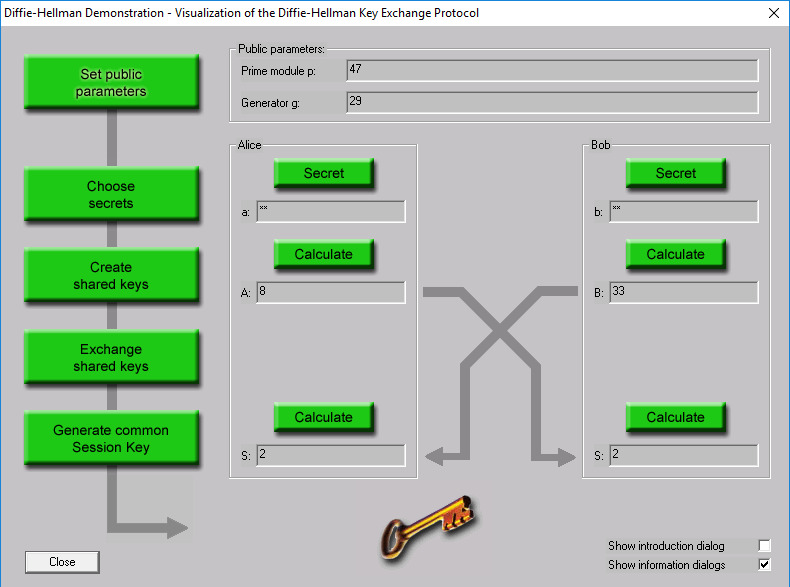
\includegraphics[scale=0.4]{4-cryptool-1}
\end{center}

Alice wybrała swoją utajnioną liczbę $a$ o wartości $16$.
Bob natomiast ustalił analogicznie liczbę $b$ o wartości $31$.

Jeśli któraś z liczb $a$ i $b$ byłaby większa lub równa od modułu $p$, to należałoby je zredukować.
W tym przypadku nie było to konieczne.

Na podstawie uprzednio wybranych liczb, Alice i Bob tworzą liczby, które wymienią miedzy sobą.

W tym przypadku, te liczby to $8$ i $33$ kolejno.

Na podstawie wymienionych miedzy sobą liczb, Alice i Bob w niezależny sposób są w stanie wyliczyć klucz sesyjny (obojgu powinien wyjść ten sam).

W przypadku tego eksperymentu, uzyskaną wartością była liczba $2$.

\subsection{Moduł dużej liczby pierwszej}

\begin{center}
	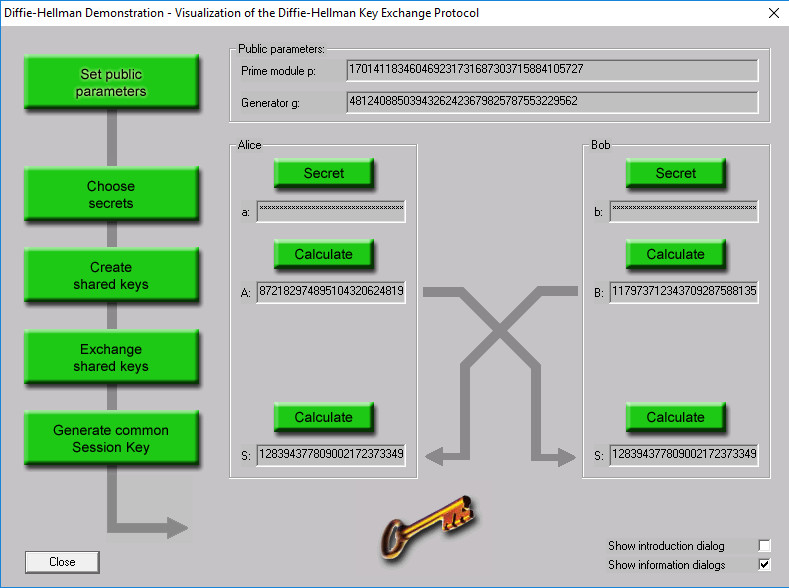
\includegraphics[scale=0.4]{4-cryptool-2}
\end{center}

\end{document}
